\documentclass[dvipdfmx, 12pt]{article}
\usepackage{mathpazo}
\usepackage{amsmath,amssymb}
\usepackage{array}
\usepackage[hiresbb]{graphicx}
\usepackage{tikz}
\usepackage{textcomp}
\usepackage{dcolumn}
\usepackage{here}
\usepackage{lscape}
\usepackage[top=25truemm,bottom=30truemm,left=25truemm,right=25truemm]
{geometry}
\begin{document}

\begin{table}[H]
  \centering
  \begin{tabular}{lcccccc}\hline
    index & type & cutpoint & binsize & bandwidth & $\theta$ & $z$
    \\ \hline \hline
    AVG & rate & .300 & .001 & .019 &  .499 & 7.442*** \\
    & & & & & (0.067) & \\
    OBP & rate & .350 & .001 & .024 &  .139 & 2.854** \\
    & & & & & (0.049) &  \\
    HR & cumulative & 20 & 1 & 5.309 & .259 & 3.465*** \\
    & & & & & (.075)  & \\
    RBI & cumulative & 100 & 4 & 15.423 & .311 & 3.295*** \\
    & & & & & (0.094) & \\
    SB & cumulative & 30 & 1 & 10.000 & .529 & 4.274*** \\
    & & & & & (.124) & \\
    & & 40 & 1 & 11.505 & .481 & 2.764** \\
    & & & & & (.174) & \\
    PA & cumulative & 500 & 1 & 0.003 & .160 & 2.515* \\
    & & & & &(.063) & \\
    H & cumulative & 200 & 1 & 18.922 & .453 & 2.547 * \\
    & & & & & (.178) & \\ \hline \hline
  \end{tabular}
  \footnotesize
  \flushright
      ***: $p<0.1\%$, **: $p<1\%$, *: $p<5\%$.

    Bandwidth is optimized following the method of Mcrary(2007).
  \normalsize
  \caption{Test for Manipulation :leastPA $= 200$}
\end{table}

\begin{figure}[H]
  \centering
  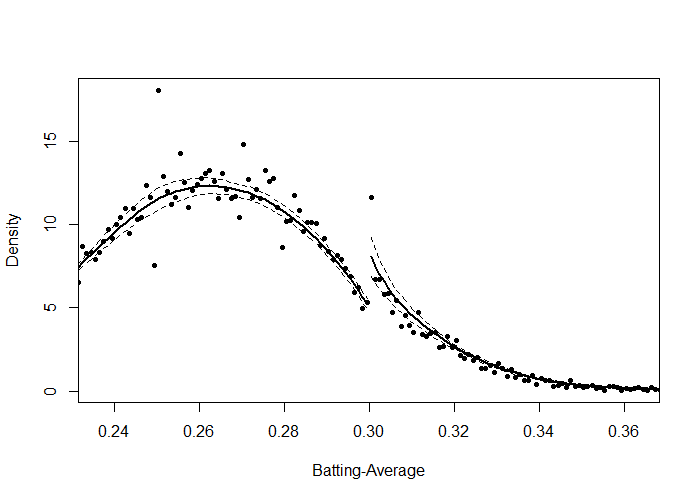
\includegraphics[width = 10cm, height = 7cm]{graphs/AVG_300.png}
  \caption{Discontinuity in AVG (at least 200PA)}
  \label{AVG_300}
\end{figure}
\begin{figure}[H]
  \centering
  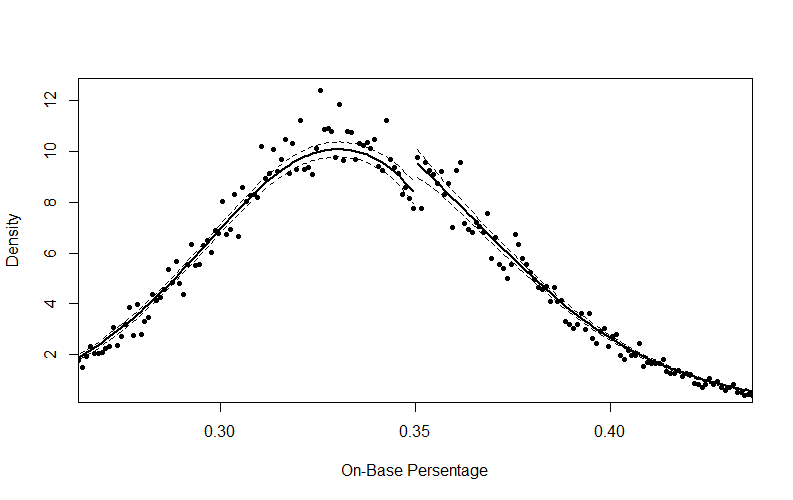
\includegraphics[width = 10cm, height = 7cm]{graphs/OBP_350.png}
  \caption{OBP (at least 200PA)}
  \label{OBP_350}
\end{figure}
\begin{figure}
  \centering
  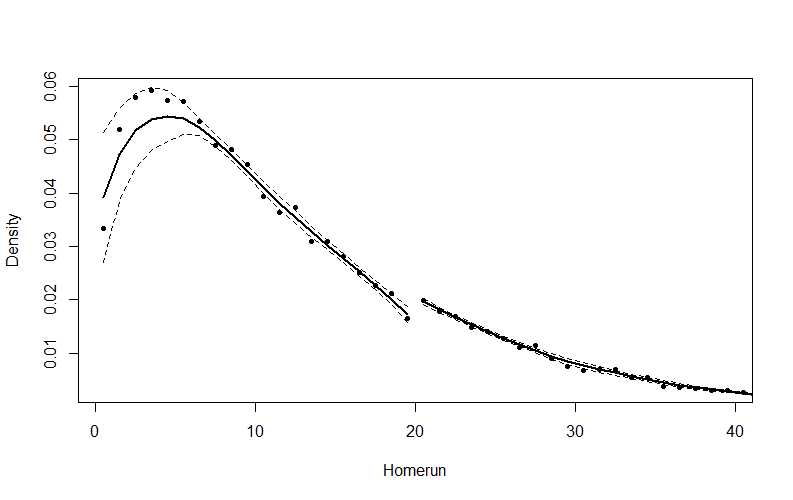
\includegraphics[width = 10cm, height = 7cm]{graphs/HR_20.png}
  \caption{HR (at least 200PA)}
  \label{HR_20}
\end{figure}
\begin{figure}[H]
  \centering
  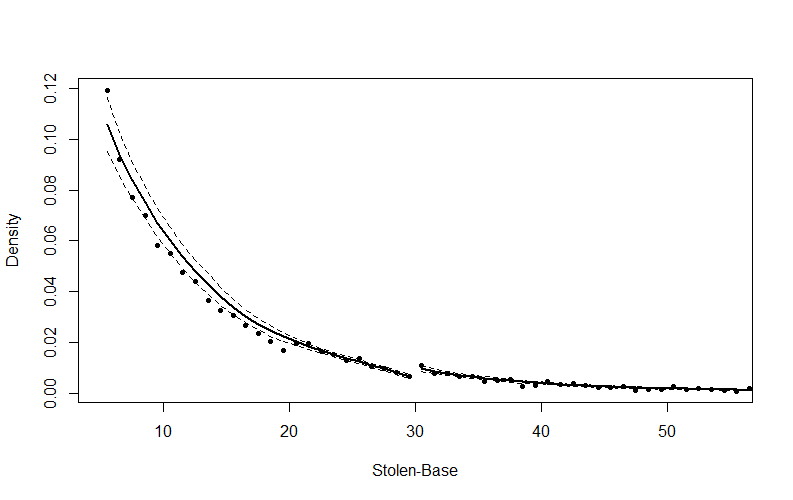
\includegraphics[width = 10cm, height = 7cm]{graphs/SB_30.png}
  \caption{SB: cutpoint $=30$ (at least 5SB)}
  \label{SB_30}
\end{figure}
\begin{figure}[H]
  \centering
  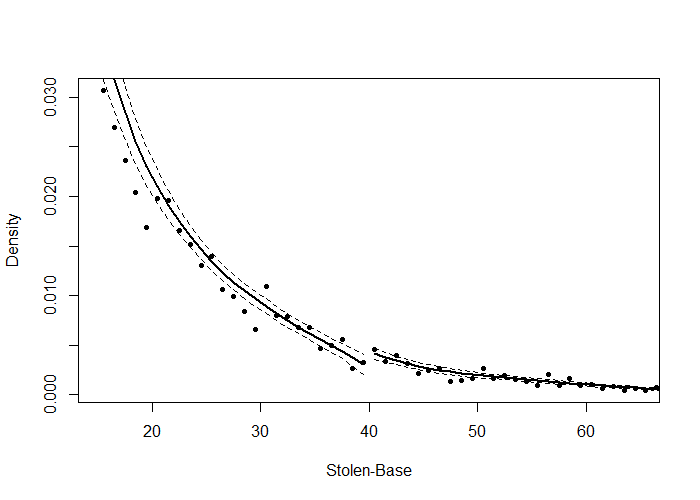
\includegraphics[width = 10cm, height = 7cm]{graphs/SB_40.png}
  \caption{SB: cutpoint $=40$ (at least 5SB)}
  \label{SB_40}
\end{figure}
\begin{figure}[H]
  \centering
  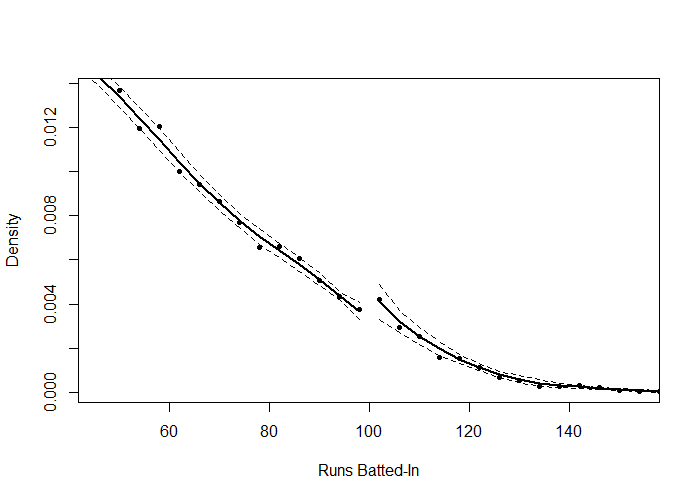
\includegraphics[width = 10cm, height = 7cm]{graphs/RBI_100.png}
  \caption{RBI (at least 200PA)}
  \label{RBI_100}
\end{figure}
\begin{figure}[H]
  \centering
  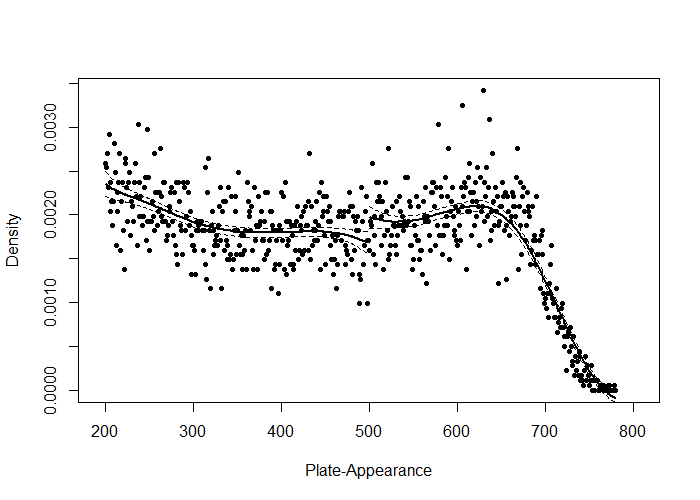
\includegraphics[width = 10cm, height = 7cm]{graphs/PA_500.png}
  \caption{PA (at least 200PA)}
  \label{PA_500}
\end{figure}
\begin{figure}[H]
  \centering
  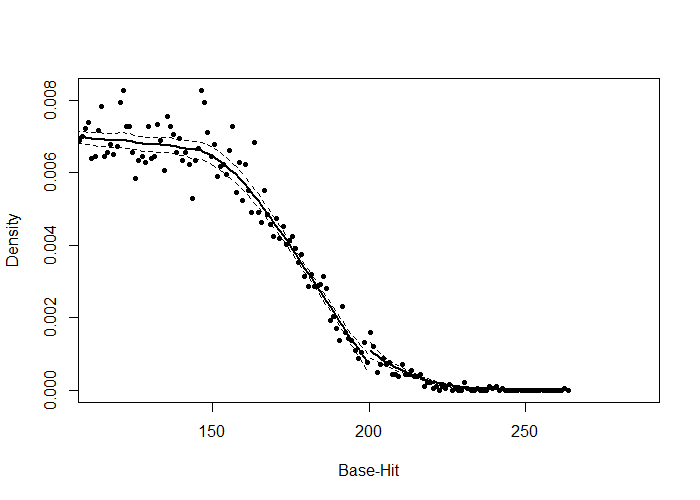
\includegraphics[width = 10cm, height = 7cm]{graphs/H_200.png}
  \caption{H (at least 200PA)}
  \label{H_200}
\end{figure}
\end{document}
